% !TEX root = ../../main.tex

% --------------------------------------
% labels: \label{mil3:res:[type]:[name]}
% --------------------------------------
% PAST TENSE


The figures below demonstrate our results for three wave numbers $k\in\{k_l, k_i, k_s\}$. We chose $k_l\equiv0.001\unit{Mpc}^{-1}$ to represent the large-scale modes and $k_s\equiv0.1\unit{Mpc}^{-1}$ for the small-scales. The intermediate-scale modes are represented by $k_i\equiv0.01\unit{Mpc}^{-1}$. We noted that $k_i\approx k\ped{eq}= 0.0115\unit{Mpc}^{-1}$.

We present the absolute values of the matter and energy perturbations in the upper panels of~\cref{mil3:res:fig:matter_perturbations}. The lower panels of said figure emphasise the oscillations around zero of the density and velocity perturbations for the photons.
\begin{figure*}[!ht]
    \begin{subfigure}{0.49\linewidth}
        \centering
        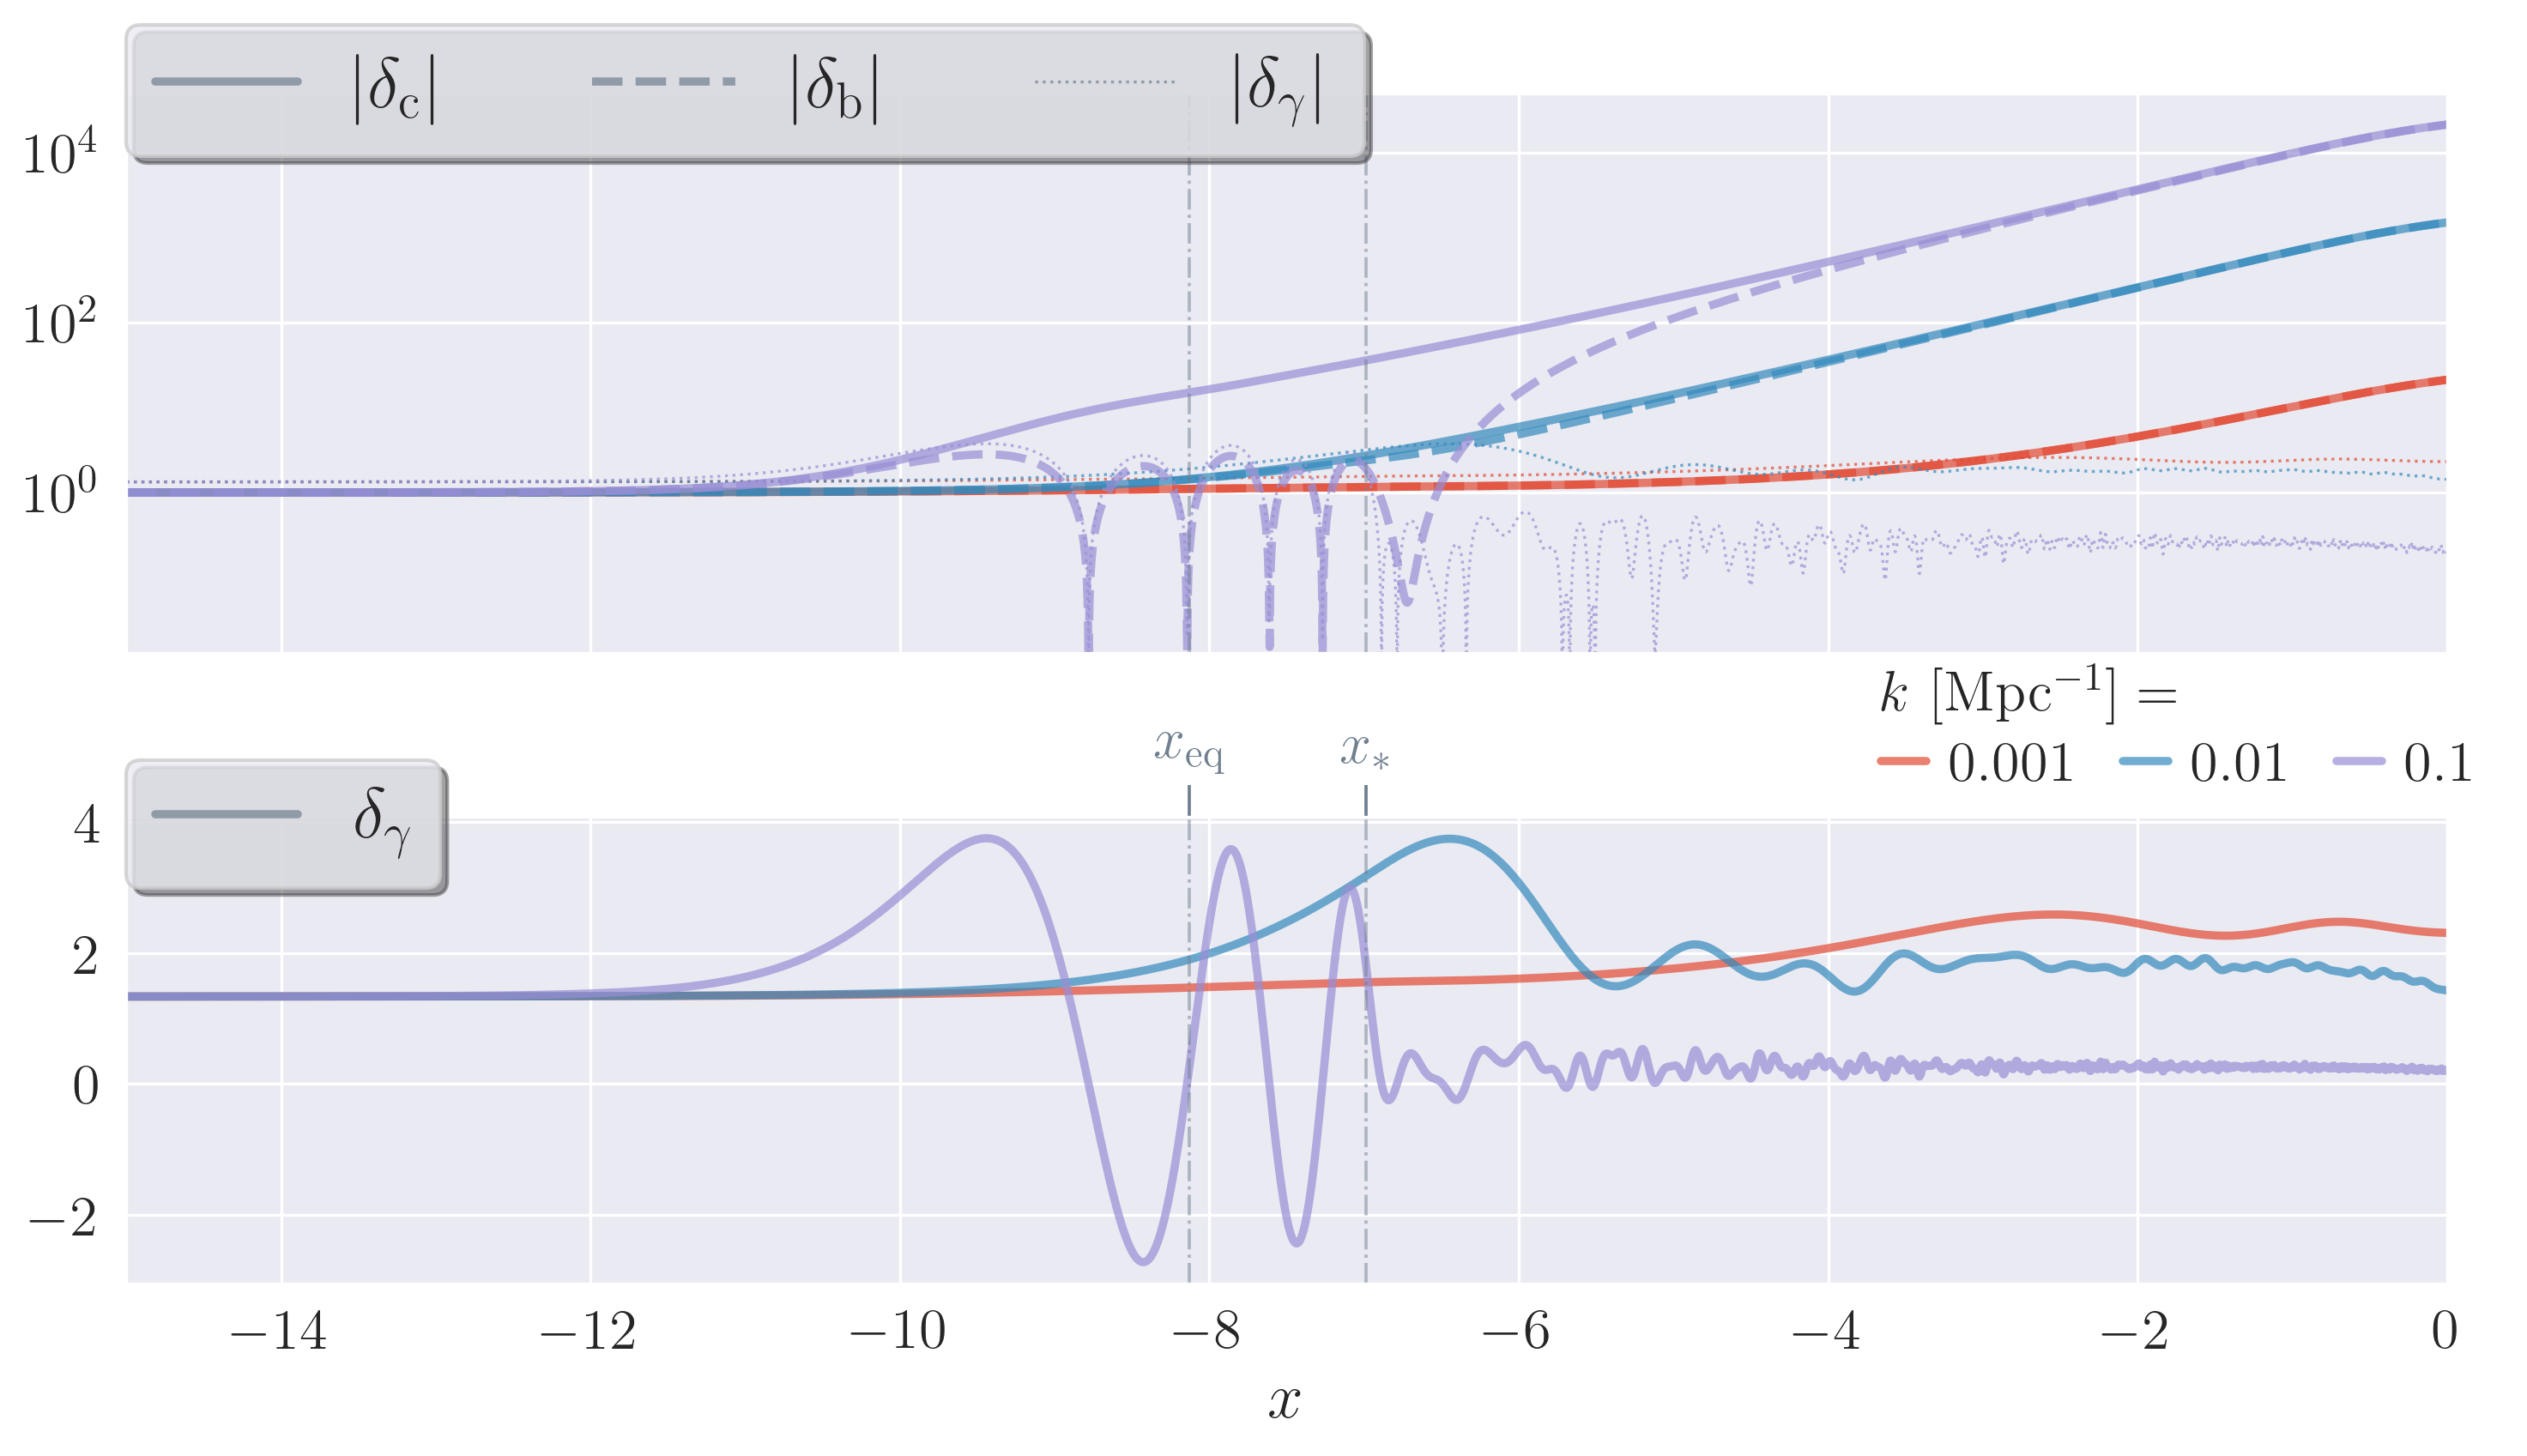
\includegraphics[width=\linewidth]{milestone3/density_perturbations.png} 
        \caption{Density perturbations $\delta_s(x, k)$ for $s=\mathrm{c,b}$ and $\gamma$ meaning cold dark matter, baryons and photons, respectively. Recall that $\delta_\gamma(x, k)=4\Theta_0(x, k)$.}
    \label[fig]{mil3:res:fig:density_perturbations}
    \end{subfigure} 
    \begin{subfigure}{0.49\linewidth}
        \centering
        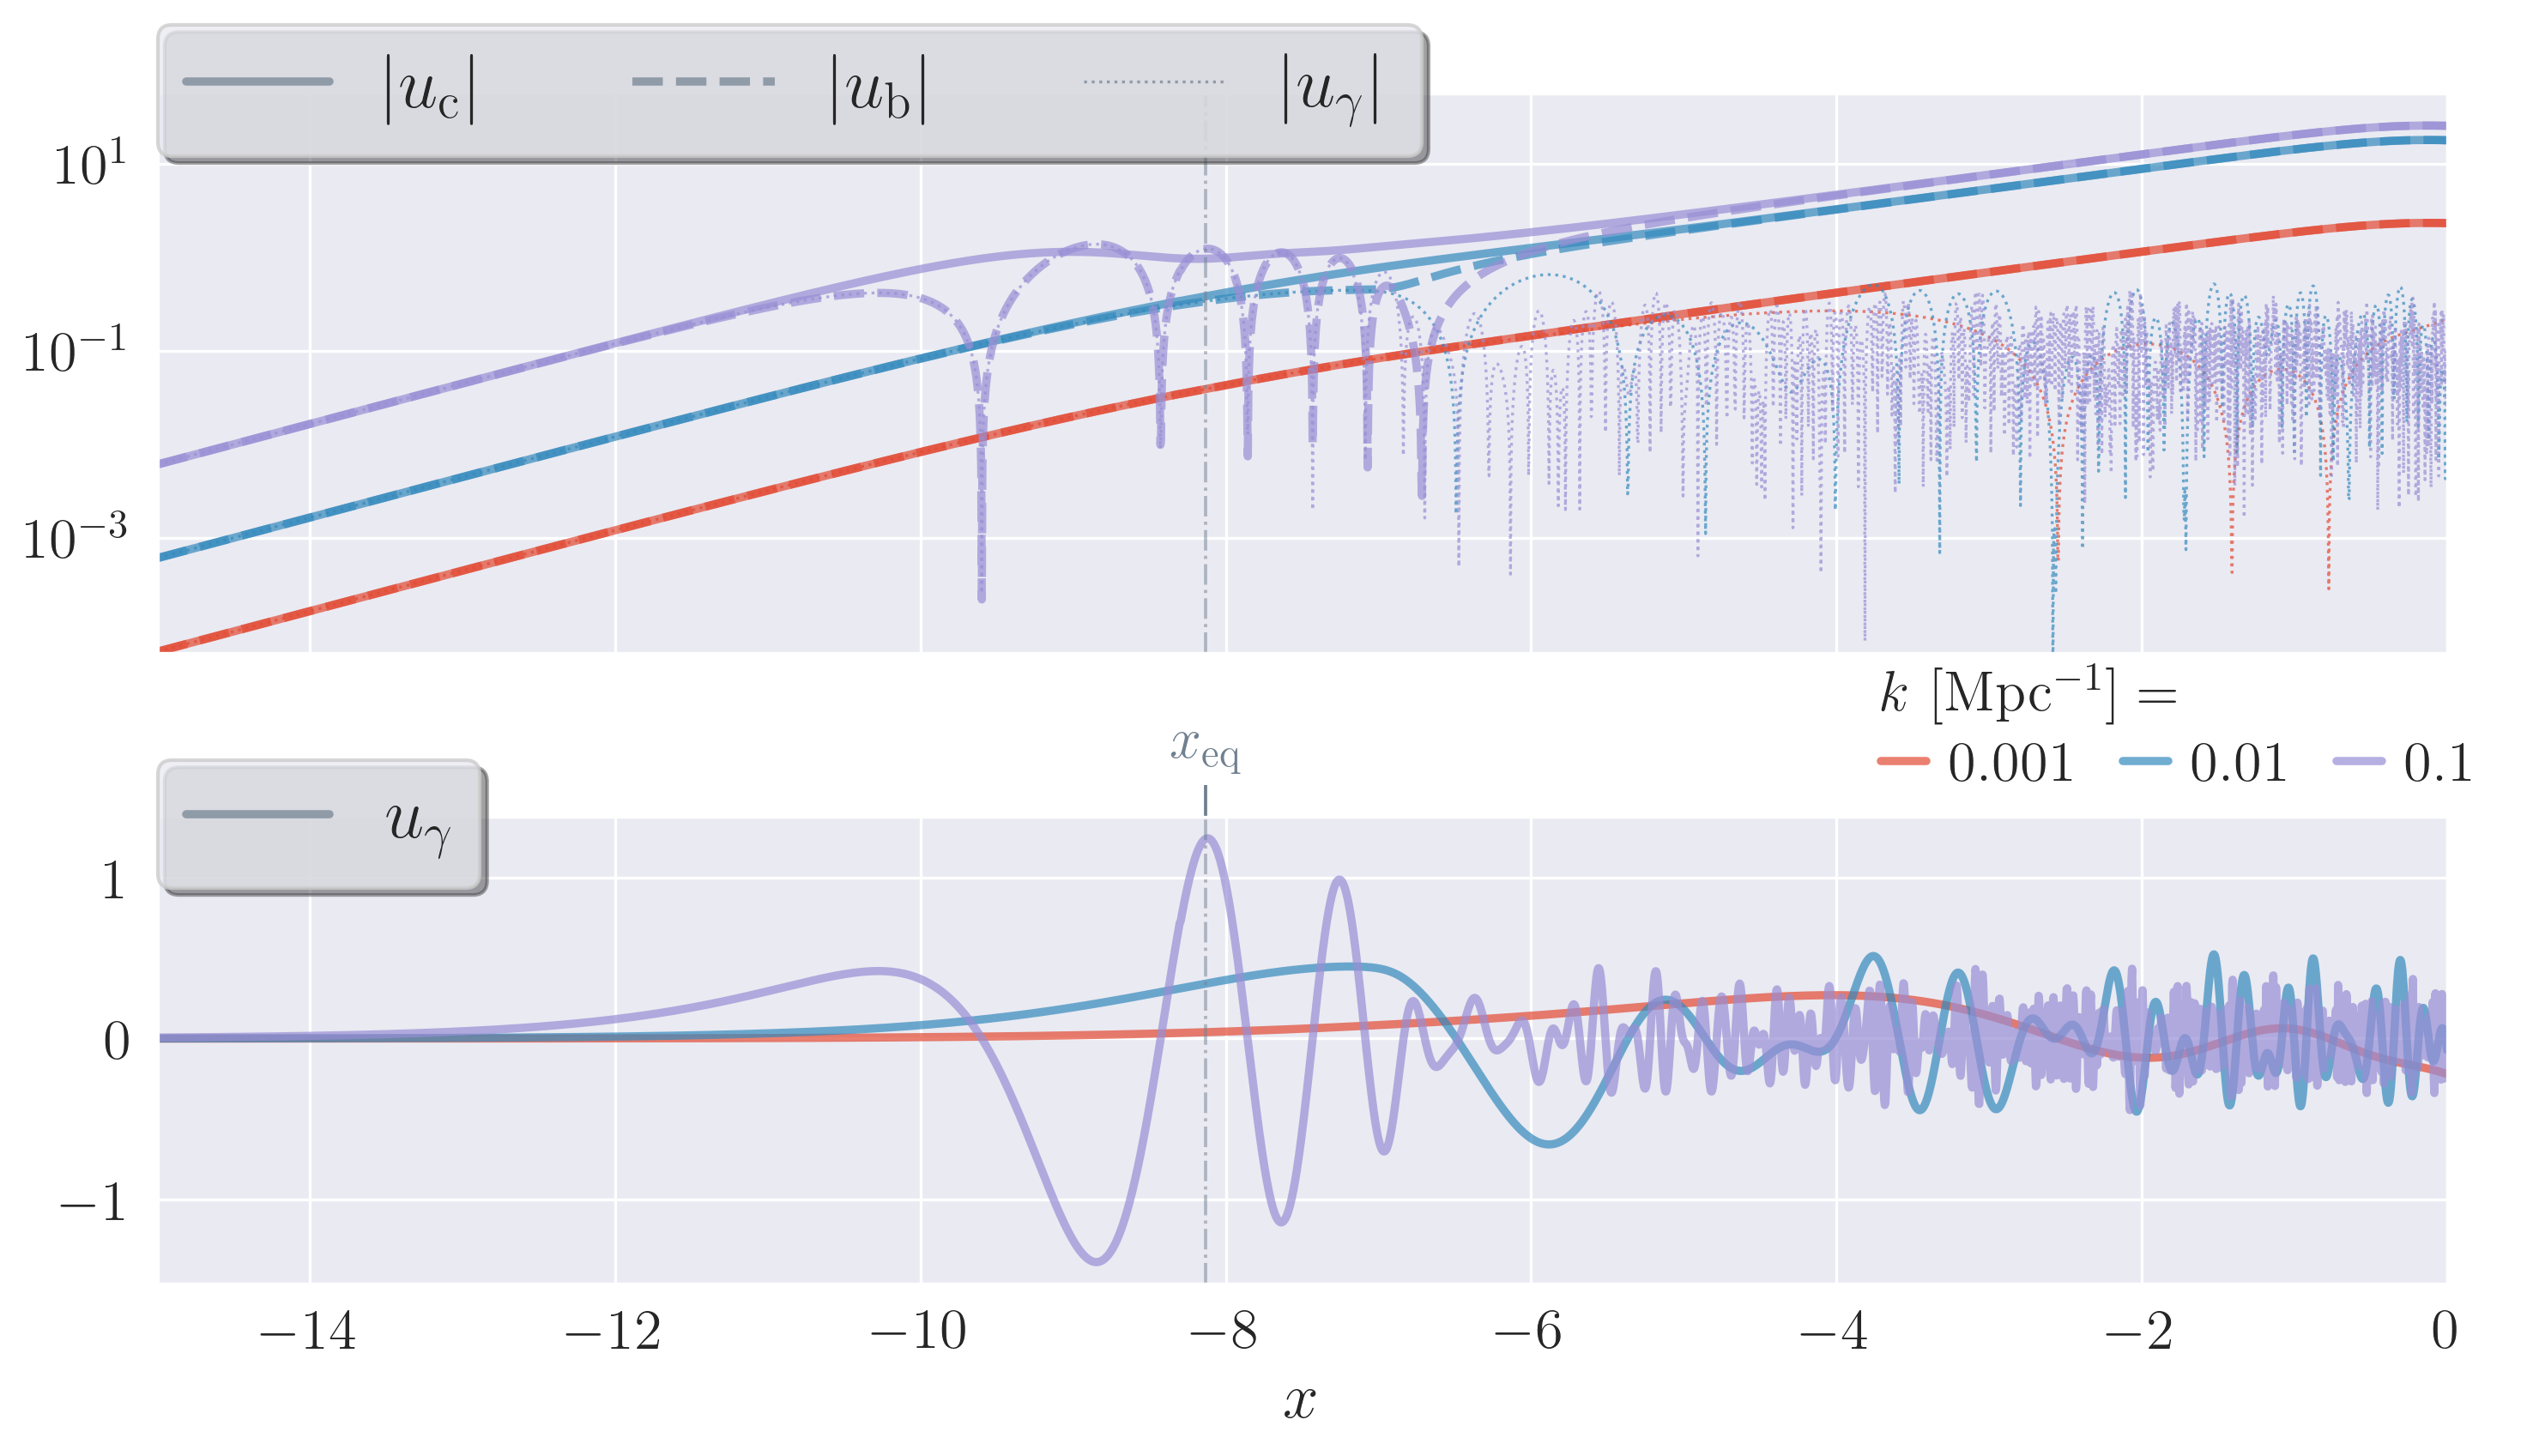
\includegraphics[width=\linewidth]{milestone3/velocity_perturbations.png} 
        \caption{Velocity perturbations $u_s(x, k)$ for $s=\mathrm{c,b}$ and $\gamma$ meaning cold dark matter, baryons and photons, respectively. Recall that $u_\gamma(x, k)=-3\Theta_1(x, k)$.} 
    \label[fig]{mil3:res:fig:velocity_perturbations}
    \end{subfigure}
    \caption{Matter perturbations to normal matter and photons as functions of logarithmic expansion $x$ for three wavenumbers $k$. The time of matter-radiation equality is marked by a vertical dash-dotted line, as is the onset of recombination. The upper panels show the absolute value of the quantities in question with a logarithmic $y$-axes, whereas the lower panels show the actual quantity for the photons only.}
\label[fig]{mil3:res:fig:matter_perturbations}
\end{figure*}

The photon quadrupole is plotted in~\cref{mil3:res:fig:photon_quadrupole}. Note that the $x$-axis is relatively short in this plot, as the function is flat until $x\sim -9$.
\begin{figure}[!ht]
    \centering
    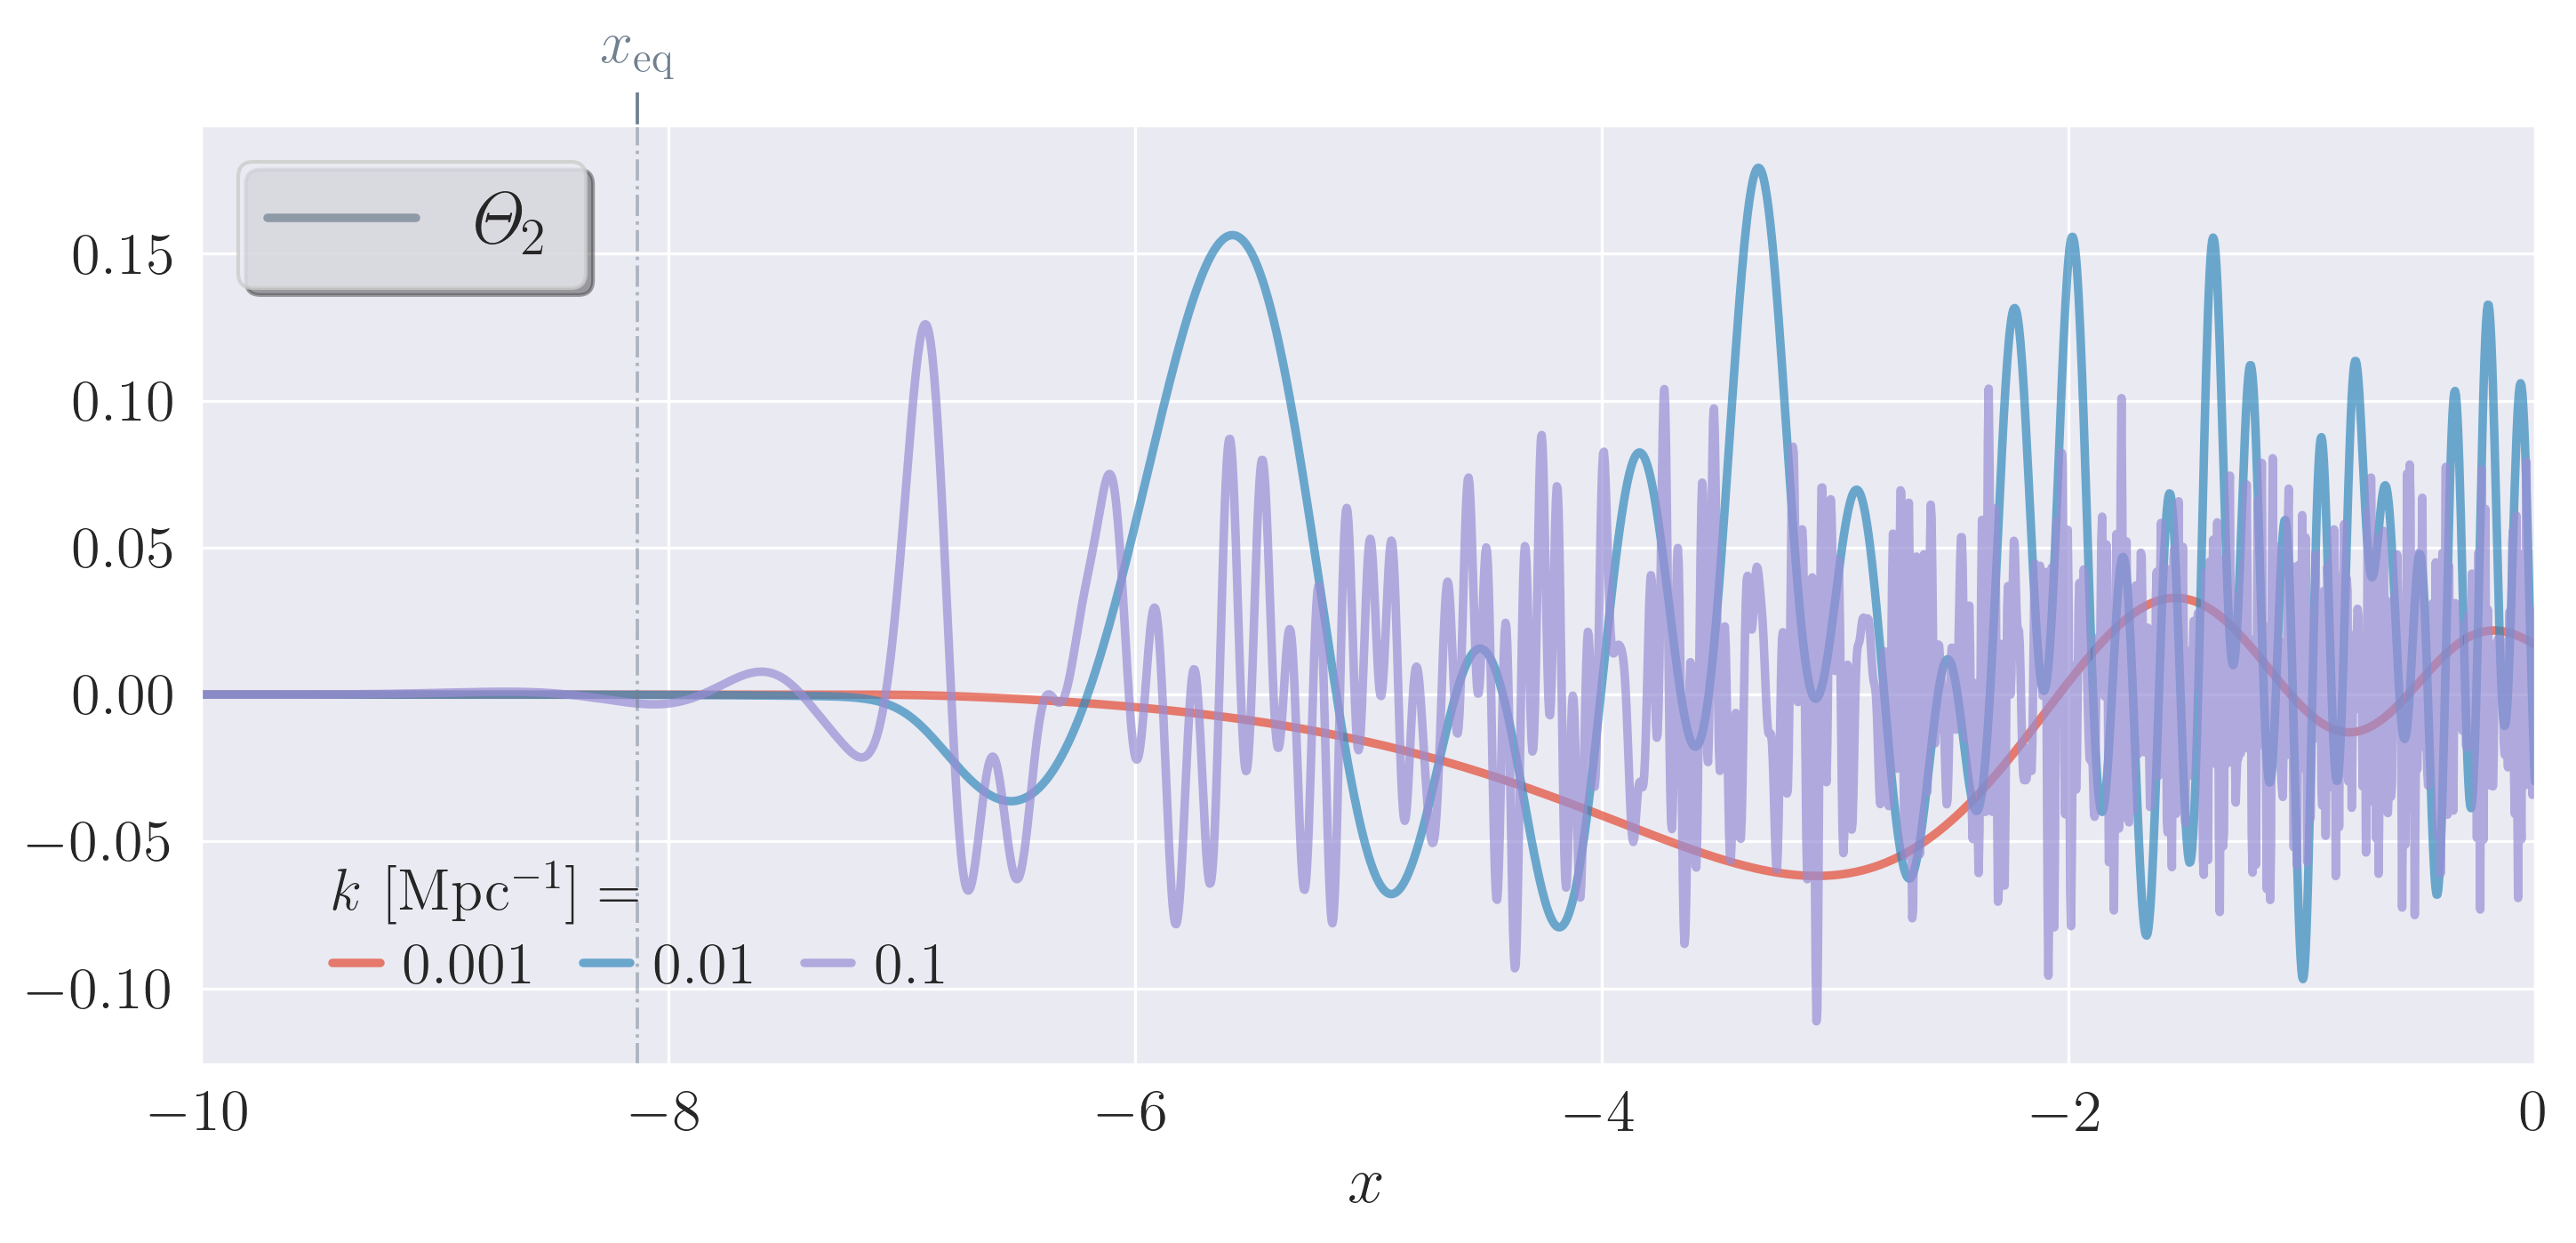
\includegraphics[width=\linewidth]{milestone3/photon_quadrupole.png} 
    \caption{The graphs show the photon quadrupole $\Theta_2(x, k)$ as function of logarithmic expansion factor $x$ for three different wavenumbers $k$. The vertical dash-dotted lines mark the time of radiation-matter equality and last scattering surface.} 
\label[fig]{mil3:res:fig:photon_quadrupole}
\end{figure}

\cref{mil3:res:fig:gravitational_potential} shows the scalar potentials as functions of time. The upper panel shows only the perturbation to the time-part of the metric, whereas the lower panel shows the sum of this and the spatial perturbation.
\begin{figure}[!ht]
    \centering
    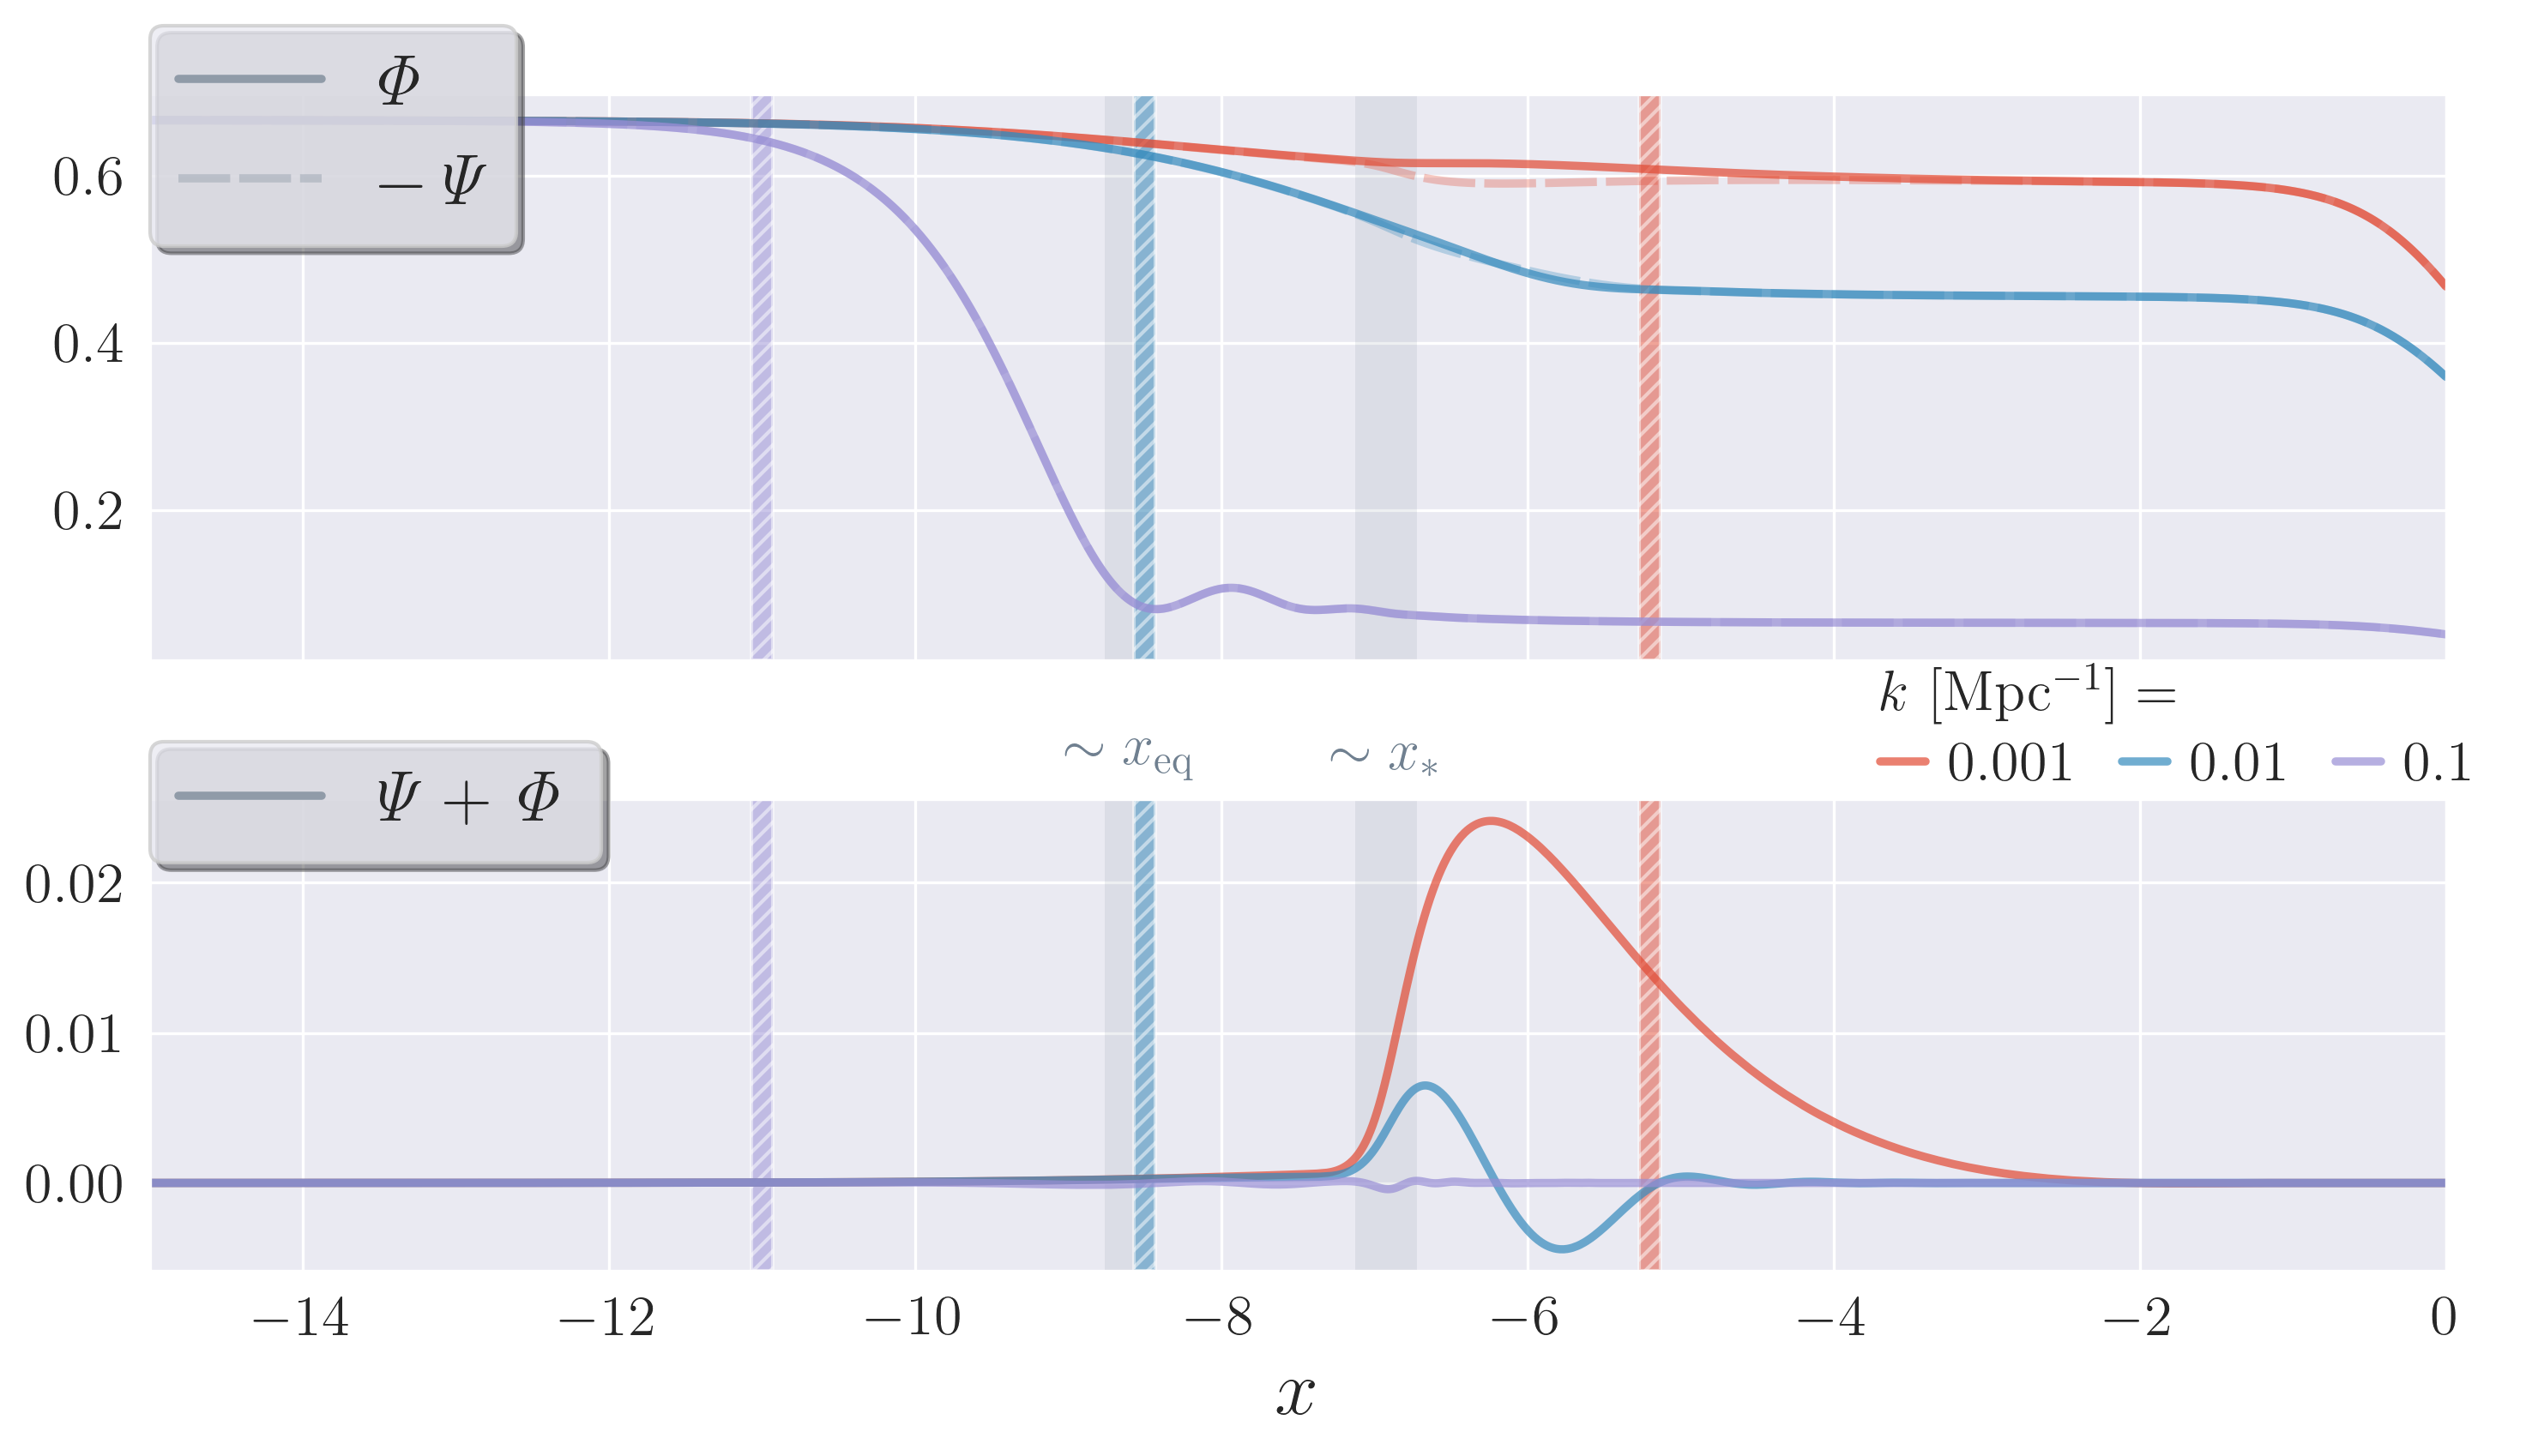
\includegraphics[width=\linewidth]{milestone3/gravitational_potential.png} 
    \caption{The graphs show the metric perturbations as functions of logarithmic expansion factor $x$ for three different wavenumbers $k$. The vertical dash-dotted lines mark the time of radiation-matter equality and last scattering surface. Upper panel: spatial curvature $\Phi(x, k)$. Lower panel: sum of the spatial curvature $\Phi(x, k)$ and the gravitational potential $\Psi(x, k)$.} 
\label[fig]{mil3:res:fig:gravitational_potential}
\end{figure}

Note that we completely dismissed neutrinos and photon polarisation. That is, we sat the effective neutrino number to be zero, slightly changing the background from \cref{sec:mil1}.

The end of tight coupling turned out to be $x\ped{tc,end}(k)=-8.3$ for all three wavenumbers. The three modes $k_s$, $k_i$ and $k_l$ entered the horizon at $x\sim -11$, $-8.3$ and $-5.1$, respectively. That is, $k_s$ enters the horizon in the radiation-dominated era, $k_i$ just around the matter-radiation equality and $k_l$ enters when the universe is dominated by matter (see~\cref{mil1:res:fig:density_params}).


